% appendix_c.tex
\chapter{Bing Pagination Screenshots}
\label{app:bing-pagination}

The following screenshots correspond to the two Bing scrapes discussed in Section~\ref{sec:bing-pagination-instability} and summarised in Tables~\ref{tab:bing-truncated}--\ref{tab:bing-full}. Both scrapes used the same query (\texttt{"free AI tools for translating video"}) and were conducted minutes apart.

\begin{figure}[htbp]
    \centering
    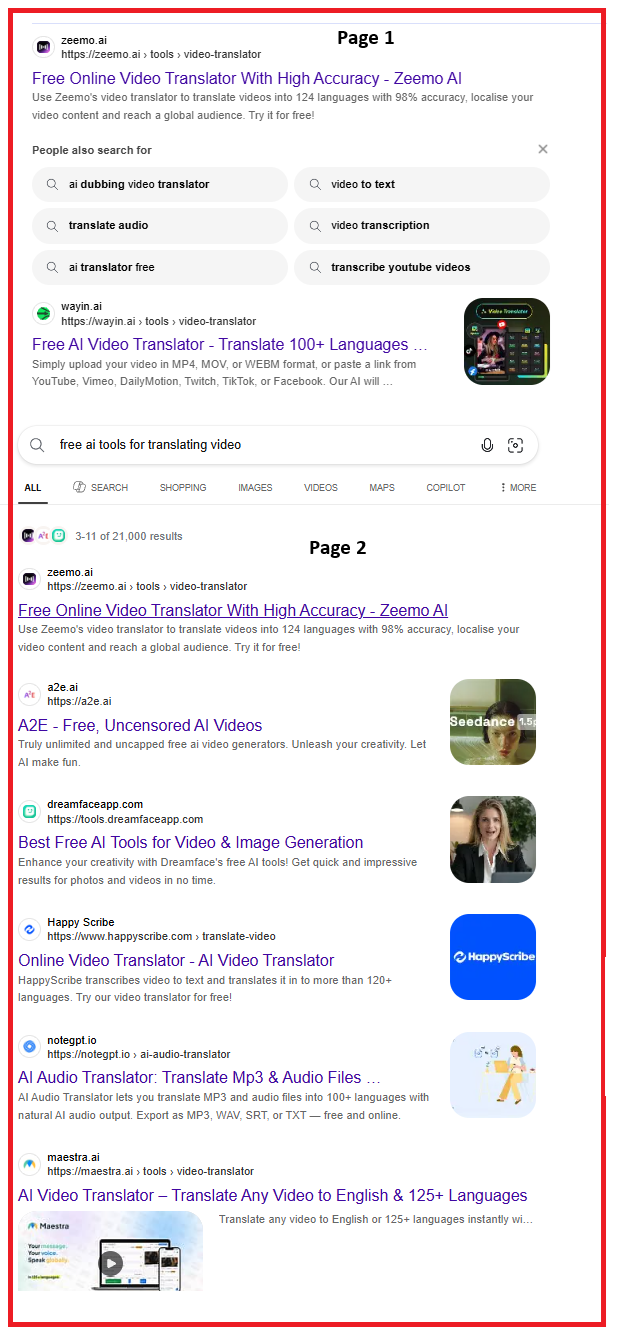
\includegraphics[width=0.75\textwidth]{figures/truncated.png}
    \caption{Truncated scrape: Page~1 (red outline) returned only 2 organic results (\texttt{zeemo.ai}, \texttt{wayin.ai}). Page~2 contained off-topic domains such as \texttt{a2e.ai} and \texttt{dreamfaceapp.com}. Ranks 3--7 from the full scrape never appeared.}
    \label{fig:bing-truncated-screenshot}
\end{figure}

\begin{figure}[htbp]
    \centering
    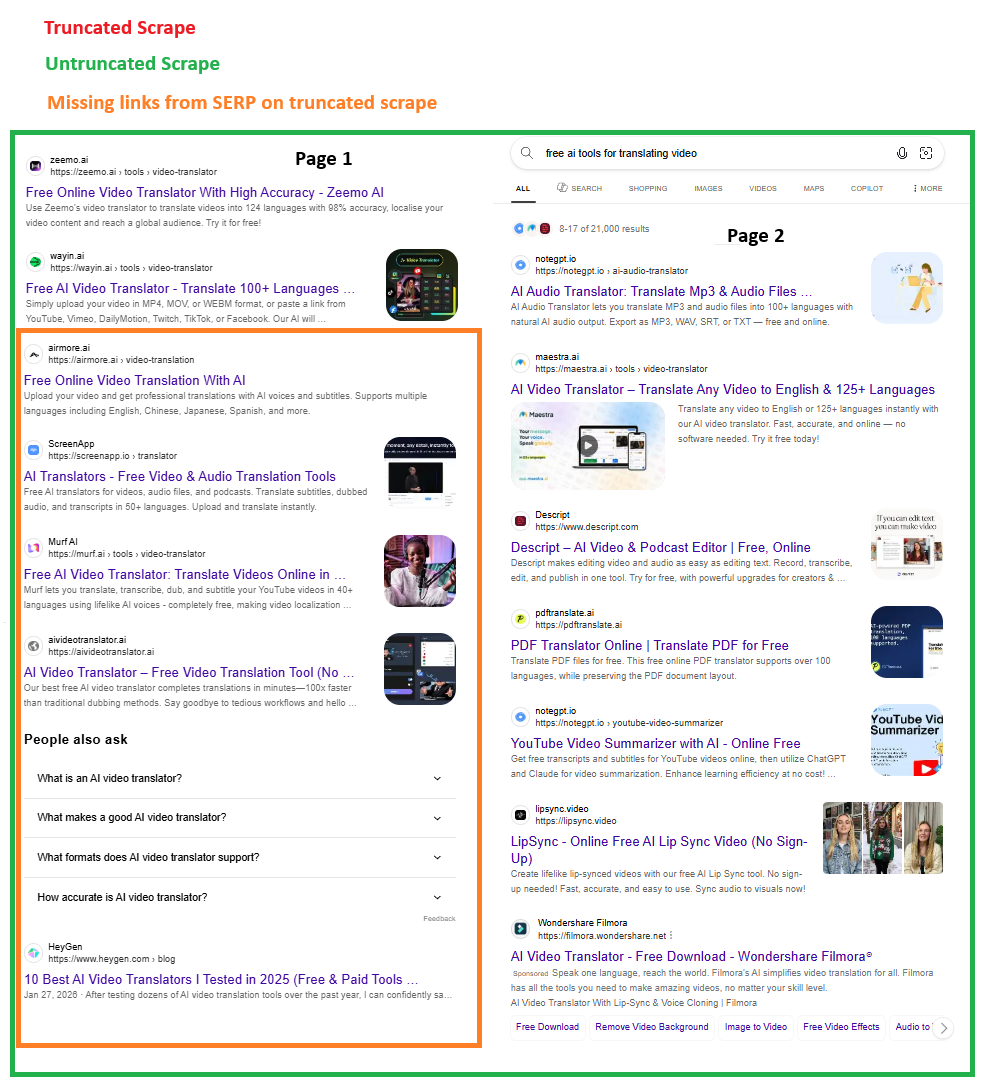
\includegraphics[width=0.75\textwidth]{figures/untruncated.png}
    \caption{Full scrape: Page~1 (green outline) returned 7+ relevant results. Orange highlights indicate ranks 3--7 (\texttt{airmore.ai}, \texttt{ScreenApp}, \texttt{Murf~AI}, \texttt{aivideotranslator.ai}, \texttt{HeyGen}) that are entirely absent from the truncated scrape's Page~2 or any subsequent depth. Page~2 (right) closely resembles the truncated scrape's Page~2, suggesting a fixed pagination offset.}
    \label{fig:bing-full-screenshot}
\end{figure}
